\documentclass[conference]{IEEEtran}
\usepackage{cite}

\usepackage{amsmath,amssymb}
\usepackage{fontspec}
\setmainfont{texgyretermes}[Extension=.otf,UprightFont=*-regular,BoldFont=*-bold,ItalicFont=*-italic,BoldItalicFont=*-bolditalic]
\usepackage{graphicx}
\usepackage{booktabs}
\usepackage{multirow}
\usepackage{xcolor}
\usepackage[hidelinks]{hyperref}
\graphicspath{{../../outputs/figures/}}

\begin{document}

\title{Statistical and Machine Learning Analytics for Patient Value, Satisfaction and Retention in a Private Outpatient Clinic: A Simulation-Based Study}

\author{\IEEEauthorblockN{Ho Van Hieu}
\IEEEauthorblockA{Student ID: 19521497 \quad Class: STAT3013.R11.CTTT, Group 10\\
University of Information Technology, Vietnam National University Ho Chi Minh City\\
Ho Chi Minh City, Vietnam\\
19521497@gm.uit.edu.vn}}

\maketitle

\begin{abstract}
Private clinics compete on both price and service experience, yet most small providers do not use their own visit records to decide where to invest. This paper builds an end-to-end analytics pipeline on a simulated outpatient clinic (5{,}000 patients, 24{,}872 visits over 2023--2025, and a 1{,}500-response satisfaction survey) and applies six families of methods to it: descriptive statistics, hypothesis tests, a two-part regression model of Patient Lifetime Value (PLV), structural equation modeling (SEM) of satisfaction and loyalty, ARIMA forecasting of weekly demand, and machine-learning classifiers for churn. Because the data-generating process is known, we can also check whether each method recovers the true effects. The two-part PLV model explains 40\% of the variance in next-year spending on held-out patients. SEM identifies doctor communication ($\beta=0.37$) and service quality ($\beta=0.35$) as the main drivers of satisfaction, which in turn drives loyalty ($\beta=0.69$), close to the true values of 0.40, 0.34 and 0.68. Weekly visits are forecast with a mean absolute percentage error of 5.8\% (ARIMA) and 4.5\% (Holt--Winters). For churn, a plain logistic regression (cross-validated AUC 0.887) matches or beats random forest, gradient boosting and a neural network. We translate these results into concrete recommendations for clinic managers.
\end{abstract}

\begin{IEEEkeywords}
Healthcare analytics, patient lifetime value, structural equation modeling, ARIMA, churn prediction, two-part model, machine learning
\end{IEEEkeywords}

%=====================================================================
\section{Introduction}
%=====================================================================
Outpatient care in Vietnam is increasingly delivered by private clinics, which earn their revenue from repeat visits and therefore behave like service businesses as much as medical providers. For such a clinic, three management questions recur: \emph{which patients are worth the most over the coming year}, \emph{what makes patients satisfied enough to come back}, and \emph{how many patients should we staff for next quarter}. Retail and telecom firms have answered similar questions for decades with customer-lifetime-value (CLV) models, satisfaction surveys and churn models~\cite{gupta2006,reichheld1990,verbeke2012}. Healthcare, by contrast, has only recently adopted these tools at scale~\cite{raghupathi2014,rajkomar2019}.

This study asks whether a single, reproducible pipeline of standard statistical and machine-learning (ML) methods can answer all three questions from the kind of data a small clinic already collects: patient registration details, visit and billing records, and a short survey. We make three contributions:
\begin{enumerate}
\item An integrated workflow that links \emph{descriptive} and \emph{inferential} statistics, a \emph{two-part regression} for PLV, \emph{SEM} for satisfaction, \emph{ARIMA} for demand and \emph{ML} for churn on one shared patient base, so that each stage feeds the next.
\item A \emph{ground-truth check}: because the data are simulated from documented rules, we report how closely each method recovers the known effects, something that real-data studies cannot do~\cite{morris2019}.
\item Practical recommendations for clinic managers, connecting survey-measured loyalty to observed return visits.
\end{enumerate}

Section~\ref{sec:related} reviews related work, Section~\ref{sec:method} describes the data and methods, Section~\ref{sec:results} presents results, Section~\ref{sec:discussion} discusses implications and limitations, and Section~\ref{sec:conclusion} concludes.

%=====================================================================
\section{Related Work}\label{sec:related}
%=====================================================================
\subsection{Customer value and churn in business}
CLV models estimate the future net value of a customer from past behaviour. Recency, frequency and monetary value (RFM) summarise that behaviour and remain strong predictors~\cite{fader2005}; Gupta \emph{et al.}~\cite{gupta2006} review the main modelling families. Churn prediction is usually framed as binary classification. Verbeke \emph{et al.}~\cite{verbeke2012} compared many classifiers on telecom data and found that comprehensible models such as logistic regression often perform close to complex ones. Reichheld and Sasser~\cite{reichheld1990} showed that small improvements in retention can raise profit substantially, which motivates retention analytics in any repeat-purchase business, clinics included.

\subsection{Healthcare analytics}
In health economics, medical expenditure is notoriously skewed and has many zeros. The \emph{two-part model} of Duan \emph{et al.}~\cite{duan1983twopart} separates the decision to use care from the amount spent, and Duan's smearing estimator~\cite{duan1983smearing} corrects the bias of re-transforming log-scale predictions. For patient demand, ARIMA and exponential-smoothing models are widely used to forecast emergency-department and clinic volumes~\cite{jones2008}. Missed appointments and non-return are an active ML application area~\cite{dantas2018}, and Rajkomar \emph{et al.}~\cite{rajkomar2019} survey ML in clinical medicine more broadly.

\subsection{Service quality, satisfaction and loyalty}
SERVQUAL~\cite{parasuraman1988} established service quality as a multi-dimensional construct measured by Likert items. SEM is the standard tool for testing how such constructs drive satisfaction and loyalty, with reliability and validity assessed by composite reliability, average variance extracted (AVE) and the Fornell--Larcker criterion~\cite{fornell1981,hair2019}, and model fit judged by CFI, TLI and RMSEA cut-offs~\cite{hu1999}.

\subsection{Research gap}
Most studies apply \emph{one} of these method families to \emph{one} question. Few combine them on a single patient base, so the link between what patients \emph{say} in surveys and what they \emph{do} afterwards is rarely tested. In addition, real-data studies cannot tell whether an estimated effect is correct. A transparent simulation addresses both gaps, and it can be replaced by real records when they become available.

%=====================================================================
\section{Methodology}\label{sec:method}
%=====================================================================
Fig.~\ref{fig:workflow} gives an overview. One simulated patient base feeds six analysis stages, and each stage follows the same sequence: data preparation, preprocessing, modeling and evaluation.

\begin{figure*}[t]
\centering
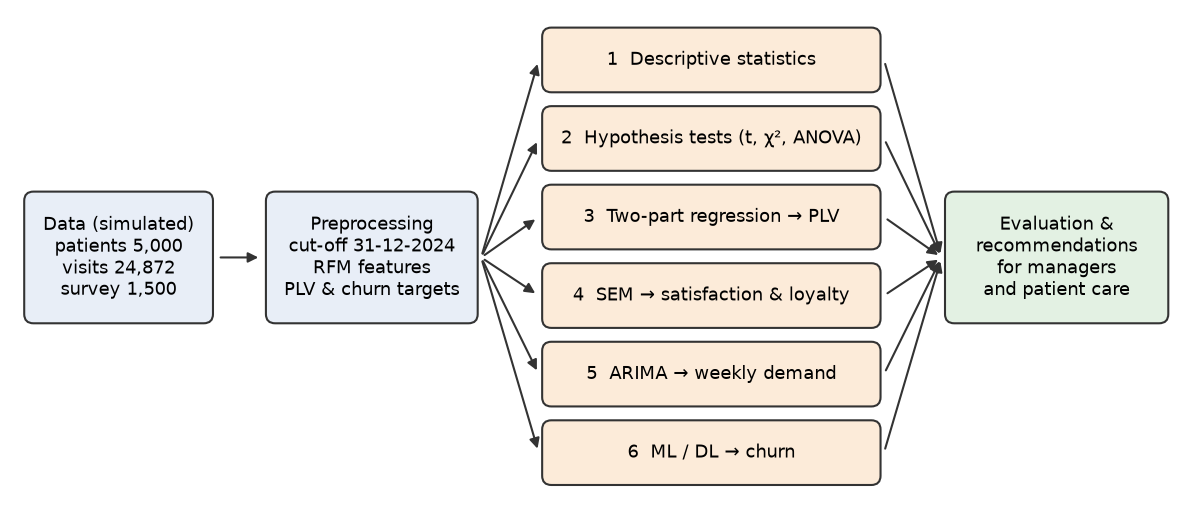
\includegraphics[width=0.85\textwidth]{f0_workflow.png}
\caption{Project workflow: one patient base feeds six analysis stages whose results are combined into recommendations.}\label{fig:workflow}
\end{figure*}
\subsection{Data}
We simulate a private outpatient clinic in Ho Chi Minh City from January 2023 to December 2025 (seed 3013; code and data are public). The data contain three tables:
\begin{itemize}
\item \textbf{Patients} ($n=5{,}000$): age, gender, public health insurance (65.6\%), chronic condition (31.4\%), membership of a follow-up care programme (29.6\%), acquisition channel and main department.
\item \textbf{Visits} ($n=24{,}872$): date, department, total cost, out-of-pocket (OOP) payment and waiting time. Visits follow a patient-specific Poisson process thinned by a flu-season cycle peaking in January, weekday effects and a Lunar New Year (Tet) closure. Each patient leaves the clinic after an exponentially distributed lifetime whose mean increases with loyalty.
\item \textbf{Survey} ($n=1{,}500$): 20 five-point Likert items for six constructs: service quality (SQ, 4 items), doctor communication (DC, 4), access and convenience (AC, 3), price fairness (PF, 3), satisfaction (SAT, 3) and loyalty intention (LOY, 3). They are generated from latent variables that also drive the patient's real lifetime.
\end{itemize}
The true structural relations, e.g. $\mathrm{SAT}=0.30\,\mathrm{SQ}+0.35\,\mathrm{DC}+0.20\,\mathrm{AC}+0.20\,\mathrm{PF}+\varepsilon$, are listed in the code so that estimates can be checked.

\subsection{Preprocessing and design}
All patient-level models use a fixed \emph{cut-off} of 31 Dec 2024. Features are computed only from visits up to the cut-off: frequency, total and average OOP spend, average waiting time, recency, tenure and number of departments. Targets are measured afterwards: \textbf{PLV} is the OOP spend during 2025, and \textbf{churn} means no visit between January and June 2025. This prevents information leakage. The resulting cohort has 3{,}070 patients, 62.4\% of whom churn and 60.2\% of whom have zero PLV. Models are trained on a stratified 80\% split and evaluated on the remaining 20\%.

\subsection{Descriptive and inferential statistics}
We report means, variances, skewness and kurtosis, and use histograms, box plots and scatter plots. Five hypotheses are tested at $\alpha=0.05$: (H1) programme members spend more per year (Welch $t$-test~\cite{welch1947}, with Mann--Whitney $U$ as a robustness check given the skew); (H2) returning is associated with insurance status, and (H2b) with chronic status ($\chi^2$ tests); (H3) returning is associated with acquisition channel ($\chi^2$); (H4) waiting time differs between departments (one-way ANOVA and Kruskal--Wallis); and (H5) programme members report higher satisfaction (Welch $t$). Effect sizes are Cohen's $d$, Cram\'er's $V$ and $\eta^2$.

\subsection{Two-part regression for PLV}
Let $Y_i$ be the PLV of patient $i$ and $\mathbf{x}_i$ the features. The two-part model~\cite{duan1983twopart} is
\begin{align}
\Pr(Y_i>0\mid\mathbf{x}_i) &= \sigma(\mathbf{x}_i^\top\boldsymbol{\gamma}),\\
\log Y_i \mid Y_i>0 &= \mathbf{x}_i^\top\boldsymbol{\beta}+u_i,\\
\widehat{\mathbb{E}}[Y_i\mid\mathbf{x}_i] &= \sigma(\mathbf{x}_i^\top\hat{\boldsymbol{\gamma}})\,
e^{\mathbf{x}_i^\top\hat{\boldsymbol{\beta}}}\,\hat{\phi},\\
\hat{\phi} &= \tfrac{1}{n_+}\textstyle\sum_{i:Y_i>0} e^{\hat u_i},
\end{align}
where $\sigma(\cdot)$ is the logistic function and $\hat\phi$ is Duan's smearing factor~\cite{duan1983smearing}. Part~2 is estimated by OLS with HC3 robust standard errors. We check the OLS assumptions with the variance inflation factor (VIF), the Breusch--Pagan test (homoscedasticity), the Jarque--Bera test (normality) and the Durbin--Watson statistic. A random forest~\cite{breiman2001} fitted directly to $Y_i$ is the non-linear benchmark.

\subsection{Structural equation modeling}
The measurement model links each item to its construct; the structural model is $\mathrm{SAT}\leftarrow\mathrm{SQ}+\mathrm{DC}+\mathrm{AC}+\mathrm{PF}$ and $\mathrm{LOY}\leftarrow\mathrm{SAT}$. It is estimated by maximum likelihood in \texttt{semopy}~\cite{semopy2020}. Reliability is assessed by Cronbach's $\alpha$ and composite reliability (CR $\ge0.7$), convergent validity by AVE ($\ge0.5$), and discriminant validity by the Fornell--Larcker criterion~\cite{fornell1981}. Fit uses CFI and TLI ($\ge0.95$) and RMSEA ($\le0.06$)~\cite{hu1999}. A single-factor model serves as Harman's test for common-method bias~\cite{podsakoff2003}. Finally, we link survey and behaviour: among respondents in the cohort, a logistic regression of actual return on the standardised loyalty score, controlling for recency.

\subsection{ARIMA forecasting}
Visits are aggregated to 155 complete weeks. Following Box--Jenkins~\cite{box2015}, we test stationarity with the augmented Dickey--Fuller (ADF) test, inspect ACF/PACF plots and fit
\begin{align}
\phi(B)(1-B)y_t &= c+\textstyle\sum_{k=1}^{2}\big[a_k\sin\tfrac{2\pi kt}{52.18}+b_k\cos\tfrac{2\pi kt}{52.18}\big]\nonumber\\
&\quad+\delta\,\mathrm{Tet}_t+\theta(B)\varepsilon_t,
\end{align}
choosing $(p,q)\in\{0,\dots,3\}^2$ by AIC. Fourier terms capture yearly seasonality with only four parameters, which suits a short series~\cite{hyndman2021}. Residuals are checked with the Ljung--Box test. The last 13 weeks form the test set; benchmarks are additive Holt--Winters~\cite{winters1960} and seasonal naive forecasts. Accuracy is measured by MAE, RMSE and MAPE.

\subsection{Machine learning for churn}
We compare logistic regression, random forest~\cite{breiman2001}, histogram gradient boosting~\cite{friedman2001} and a multi-layer perceptron (MLP; two hidden layers of 64 and 32 ReLU units, early stopping) implemented in scikit-learn~\cite{pedregosa2011}. Numeric features are standardised and categorical features one-hot encoded inside a pipeline, so no test information leaks into training. Models are compared by 5-fold stratified cross-validated AUC, and by test-set accuracy, precision, sensitivity, specificity and F1 at a threshold of 0.5. Permutation importance explains the best model.

%=====================================================================
\section{Results}\label{sec:results}
%=====================================================================
\subsection{Descriptive statistics}
Table~\ref{tab:desc} summarises the main variables. Costs, waiting times and PLV are all right-skewed (skewness 1.7--3.1), which motivates the log transformation and non-parametric robustness checks (Fig.~\ref{fig:hist}). Cardiology is the most expensive department and General Medicine has the longest waits (Fig.~\ref{fig:box}). Median PLV is zero, because 60\% of the cohort does not spend anything in 2025. Fig.~\ref{fig:weekly} shows weekly visits growing from about 50 to 300, with a winter peak, a mid-year trough and sharp Tet drops.

\begin{table}[t]
\caption{Descriptive statistics of key variables}\label{tab:desc}
\centering\footnotesize
\setlength{\tabcolsep}{4pt}
\begin{tabular}{@{}lrrrrr@{}}
\toprule
Variable & $N$ & Mean & SD & Median & Skew\\
\midrule
Age (years) & 5000 & 42.2 & 14.2 & 42 & 0.25\\
Visit cost (k VND) & 24872 & 694.6 & 420.0 & 597 & 1.70\\
Out-of-pocket (k VND) & 24872 & 489.0 & 331.3 & 404 & 2.01\\
Waiting time (min) & 24872 & 29.1 & 20.0 & 24.6 & 1.65\\
Visits/patient to 2024 & 3070 & 4.3 & 4.0 & 3 & 2.20\\
PLV 2025 (k VND) & 3070 & 942.0 & 1817.9 & 0 & 3.09\\
\bottomrule
\end{tabular}
\end{table}

\begin{figure*}[t]
\centering
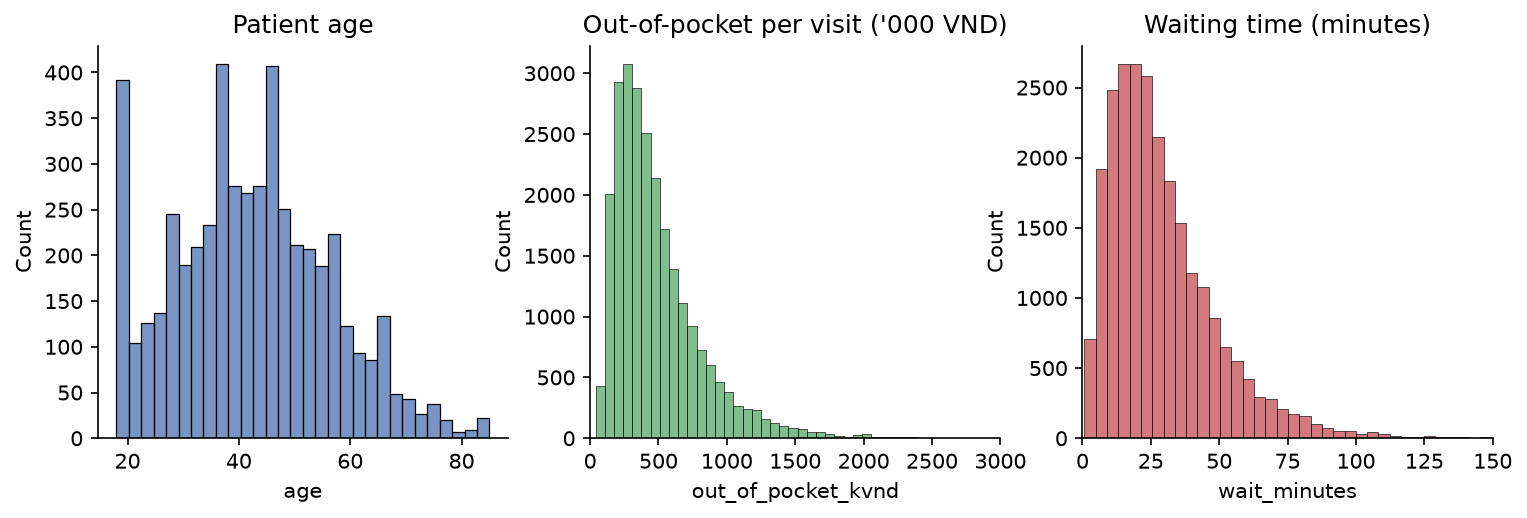
\includegraphics[width=0.9\textwidth]{f1_histograms.png}
\caption{Distributions of patient age, out-of-pocket payment per visit and waiting time.}\label{fig:hist}
\end{figure*}

\begin{figure}[t]
\centering
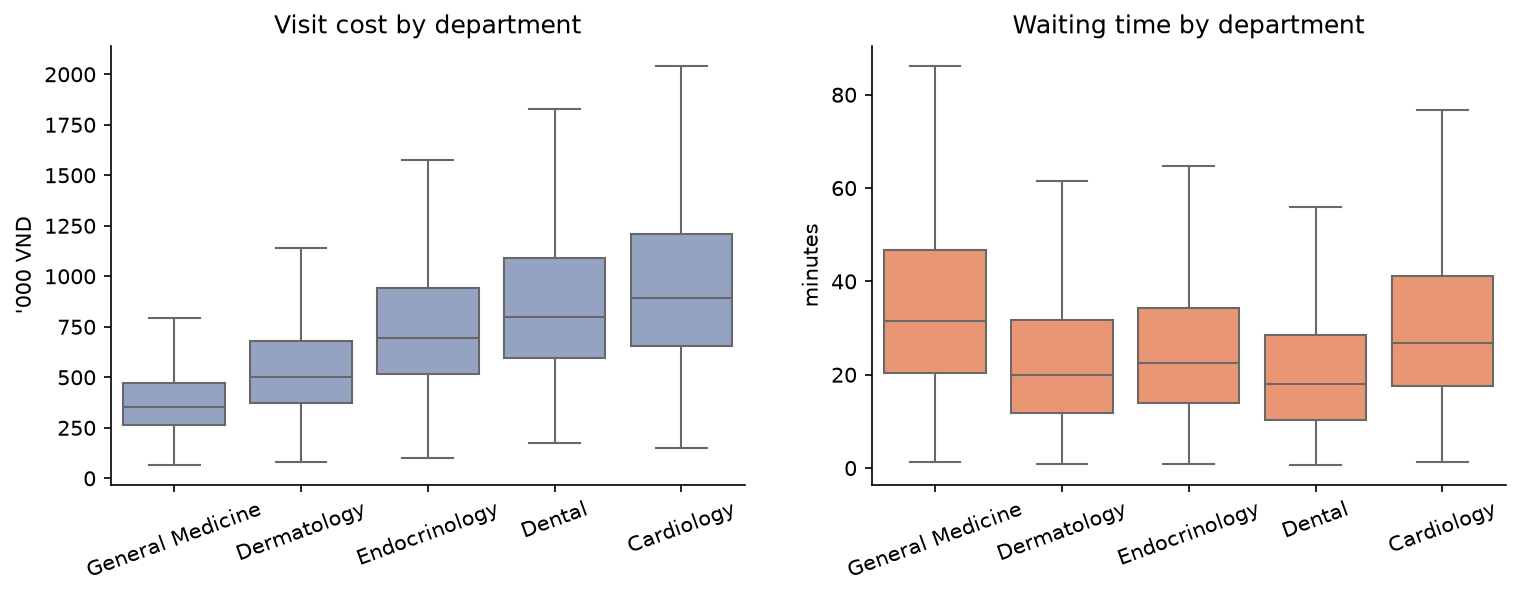
\includegraphics[width=\columnwidth]{f2_boxplots.png}
\caption{Visit cost and waiting time by department (outliers hidden).}\label{fig:box}
\end{figure}

\begin{figure}[t]
\centering
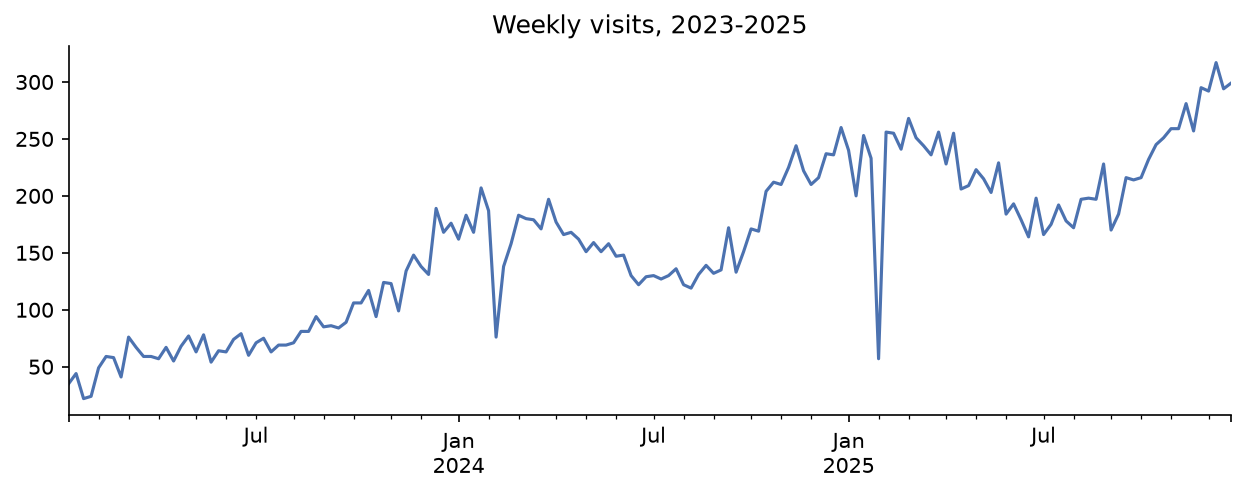
\includegraphics[width=\columnwidth]{f4_weekly_visits.png}
\caption{Weekly visits, 2023--2025: growth, seasonality and Tet drops.}\label{fig:weekly}
\end{figure}

\subsection{Hypothesis tests}
Table~\ref{tab:tests} lists the results. Programme members spent 1.82 vs 1.09 million VND in 2024 (H1, $d=0.37$). Chronic patients were much more likely to return (48.7\% vs 32.6\%, H2b). Waiting time differs between departments (H4), although the effect is modest ($\eta^2=0.073$). Insurance (H2), acquisition channel (H3) and programme membership (H5) show no significant association with returning or with satisfaction. For H5 this matches the simulation: the programme's true effect on satisfaction runs only through price fairness and is very small (about 0.06 SD).

\begin{table}[t]
\caption{Hypothesis test results ($\alpha=0.05$)}\label{tab:tests}
\centering\footnotesize
\begin{tabular}{@{}llrll@{}}
\toprule
H & Test & Statistic & $p$ & Effect\\
\midrule
H1 & Welch $t$ & 5.63 & $<.001$ & $d=0.37$\\
H1 & Mann--Whitney $U$ & 246923 & $<.001$ & --\\
H2 & $\chi^2(1)$ & 1.58 & .208 & $V=0.02$\\
H2b & $\chi^2(1)$ & 72.46 & $<.001$ & $V=0.15$\\
H3 & $\chi^2(2)$ & 0.25 & .882 & $V=0.01$\\
H4 & ANOVA $F$ & 491.6 & $<.001$ & $\eta^2=0.073$\\
H4 & Kruskal--Wallis $H$ & 2141.8 & $<.001$ & --\\
H5 & Welch $t$ & 0.19 & .852 & $d=0.01$\\
\bottomrule
\end{tabular}
\end{table}

\subsection{Patient Lifetime Value}
Part~1 (logit, pseudo-$R^2=0.41$) shows that recency dominates the decision to return: each extra month since the last visit multiplies the odds of any 2025 spending by 0.61. Chronic status (OR $1.38$) and programme membership (OR $1.34$) increase it. In Part~2 ($n=978$, $R^2=0.29$), conditional spending is 74\% higher for chronic patients, 30\% higher for programme members and 25\% lower for insured patients (all $p<.001$). Past frequency and average spend also have significant positive effects (Fig.~\ref{fig:coef}). Table~\ref{tab:twopart} lists the main coefficients of both parts. These signs and magnitudes agree with the simulation rules. For example, the true chronic visit-rate multiplier $e^{0.6}=1.82$ lies inside the 95\% CI of the estimate ($+53\%$ to $+98\%$). The insurance effect is smaller than the pure 40\% price discount because insured patients also stay slightly longer.

Diagnostics are acceptable: the maximum VIF is 3.9, Durbin--Watson is 2.00, and the residuals are only mildly skewed ($-0.57$). Breusch--Pagan ($p=.043$) indicates mild heteroscedasticity, which is why HC3 standard errors are used. On the test set (Table~\ref{tab:plv}) the two-part model reaches $R^2=0.40$, on par with the random forest and far ahead of the mean baseline. Ranking quality is high: patients in the top predicted decile spent 3.93 million VND on average in 2025, against 0 in the bottom decile (Fig.~\ref{fig:plvdiag}).

\begin{table}[t]
\caption{Two-part PLV model: selected coefficients}\label{tab:twopart}
\centering\footnotesize
\setlength{\tabcolsep}{4pt}
\begin{tabular}{@{}lrrrr@{}}
\toprule
& \multicolumn{2}{c}{Part 1: logit} & \multicolumn{2}{c}{Part 2: log-OLS}\\
\cmidrule(lr){2-3}\cmidrule(l){4-5}
Variable & OR & $p$ & $\%\Delta$ & $p$\\
\midrule
Insured & 1.29 & .055 & $-24.7$ & $<.001$\\
Chronic condition & 1.38 & .021 & $+74.2$ & $<.001$\\
Care programme & 1.34 & .020 & $+30.2$ & $<.001$\\
Age (per year) & 1.00 & .955 & $+0.5$ & .020\\
log frequency & 0.84 & .176 & $+27.6$ & $<.001$\\
log average spend & 1.17 & .230 & $+50.7$ & $<.001$\\
Recency (per month) & 0.61 & $<.001$ & $+2.1$ & .153\\
Tenure (per month) & 1.04 & .025 & $-3.1$ & $<.001$\\
Average wait (per min) & 1.00 & .939 & $-0.1$ & .544\\
\midrule
Fit & \multicolumn{2}{c}{pseudo-$R^2=0.41$} & \multicolumn{2}{c}{$R^2=0.29$, $n=978$}\\
\bottomrule
\end{tabular}
\end{table}

\begin{table}[t]
\caption{PLV prediction on the test set (k VND)}\label{tab:plv}
\centering\footnotesize
\begin{tabular}{@{}lrrrr@{}}
\toprule
Model & RMSE & MAE & $R^2$ & Spearman $\rho$\\
\midrule
Mean baseline & 1835.6 & 1277.9 & $-0.00$ & --\\
Two-part model & \textbf{1421.9} & \textbf{793.6} & \textbf{0.399} & 0.672\\
Random forest & 1428.5 & 800.1 & 0.393 & \textbf{0.693}\\
\bottomrule
\end{tabular}
\end{table}

\begin{figure}[t]
\centering
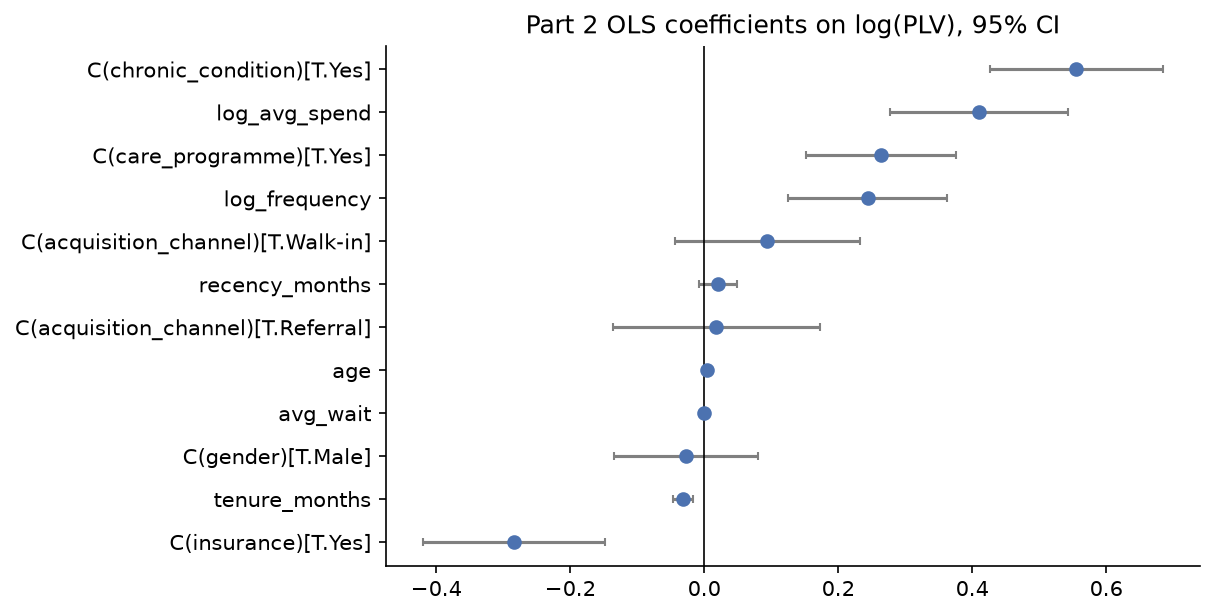
\includegraphics[width=\columnwidth]{f7_plv_coefficients.png}
\caption{Part~2 OLS coefficients on $\log(\mathrm{PLV})$ with 95\% CIs.}\label{fig:coef}
\end{figure}

\begin{figure*}[t]
\centering
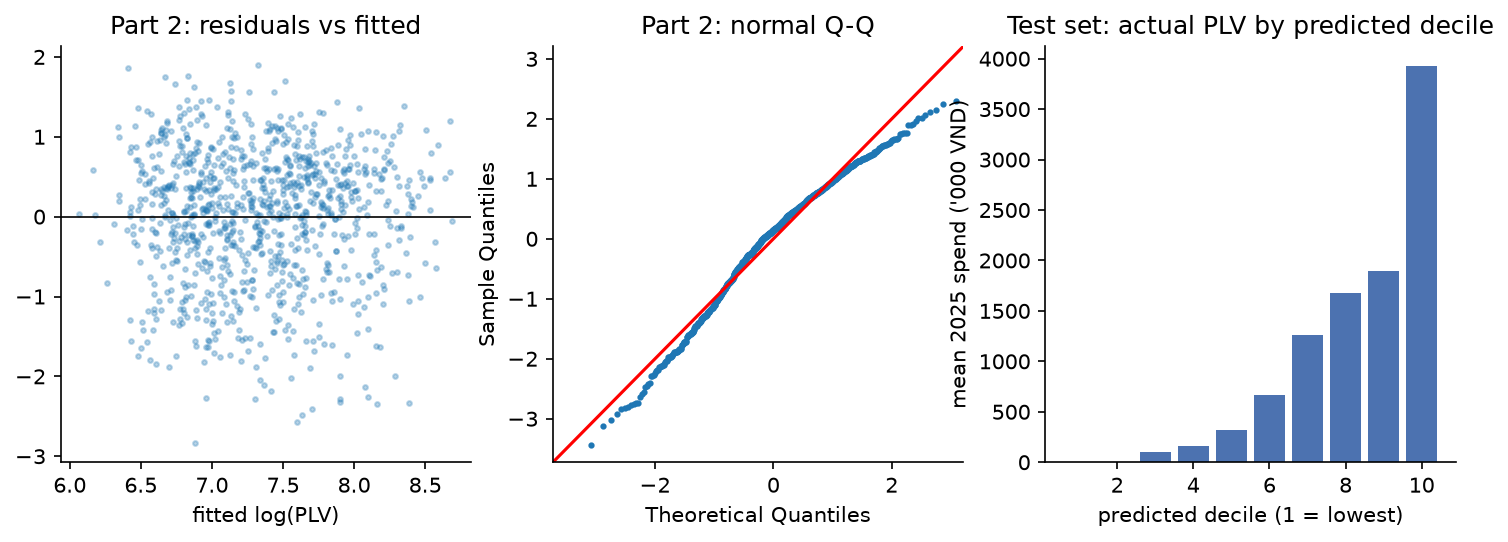
\includegraphics[width=0.9\textwidth]{f6_plv_diagnostics.png}
\caption{PLV model: residuals vs fitted, normal Q--Q plot, and mean actual PLV by predicted decile on the test set.}\label{fig:plvdiag}
\end{figure*}

\subsection{Structural equation model}
All constructs are reliable ($\alpha$ and CR between 0.74 and 0.83, all standardised loadings $\ge0.65$). AVE exceeds 0.5 for every construct except AC (0.48), which is acceptable because its CR exceeds 0.7~\cite{fornell1981}. The Fornell--Larcker criterion holds: the largest inter-construct correlation (SAT--LOY, 0.55) is below every $\sqrt{\mathrm{AVE}}$. Model fit is excellent ($\chi^2(159)=157.8$, $p=.51$; CFI $=1.00$; TLI $=1.00$; RMSEA $=0.000$), while the single-factor model fits poorly (CFI $=0.50$, RMSEA $=0.143$), so common-method bias is not a concern. The perfect fit is expected because the survey was generated from exactly this structure; with real data, a CFI near 0.95 would be typical.

Table~\ref{tab:rel} summarises the measurement quality. Fig.~\ref{fig:sem} and Table~\ref{tab:sem} show the paths. All are significant ($p<.001$), and the estimates are within 0.04 of the true standardised values. SAT explains 48\% of the variance in LOY. Most importantly, stated loyalty predicts behaviour: among 1{,}028 respondents in the cohort, one standard deviation of loyalty raises the odds of returning in early 2025 by a factor of 1.60 ($p<.001$), even after controlling for recency.

\begin{table}[t]
\caption{Measurement model: reliability and validity}\label{tab:rel}
\centering\footnotesize
\begin{tabular}{@{}lrrrrr@{}}
\toprule
Construct & Items & $\alpha$ & CR & AVE & $\sqrt{\mathrm{AVE}}$\\
\midrule
Service quality (SQ) & 4 & 0.820 & 0.821 & 0.536 & 0.732\\
Doctor communication (DC) & 4 & 0.824 & 0.826 & 0.544 & 0.738\\
Access \& convenience (AC) & 3 & 0.735 & 0.736 & 0.483 & 0.695\\
Price fairness (PF) & 3 & 0.769 & 0.771 & 0.531 & 0.729\\
Satisfaction (SAT) & 3 & 0.822 & 0.822 & 0.607 & 0.779\\
Loyalty intention (LOY) & 3 & 0.775 & 0.776 & 0.537 & 0.733\\
\bottomrule
\end{tabular}
\end{table}

\begin{figure}[t]
\centering
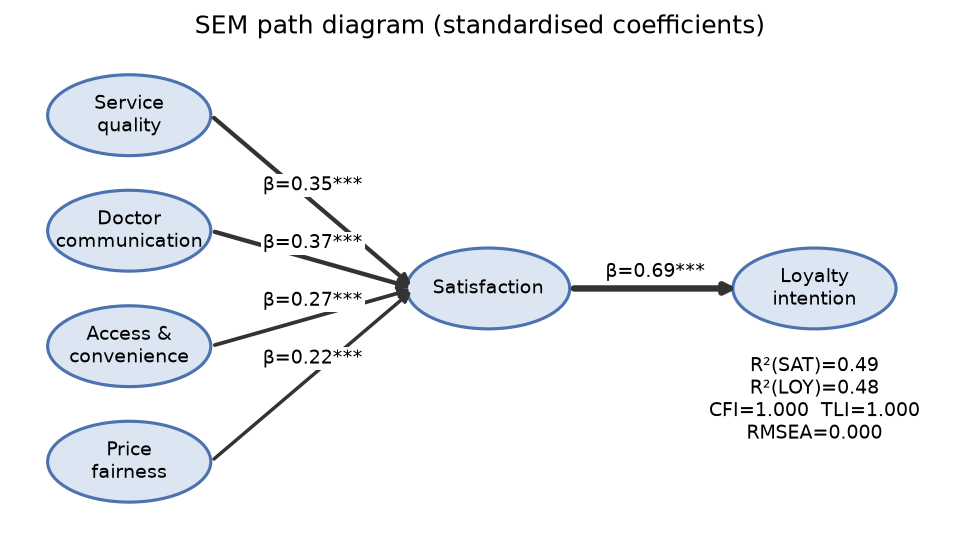
\includegraphics[width=\columnwidth]{f8_sem_path_diagram.png}
\caption{SEM path diagram with standardised coefficients (*** $p<.001$).}\label{fig:sem}
\end{figure}

\begin{table}[t]
\caption{SEM paths: estimated vs true standardised coefficients}\label{tab:sem}
\centering\footnotesize
\begin{tabular}{@{}lrrrr@{}}
\toprule
Path & Estimate & SE & True & Abs. error\\
\midrule
SAT $\leftarrow$ SQ & 0.347 & 0.033 & 0.341 & 0.006\\
SAT $\leftarrow$ DC & 0.366 & 0.031 & 0.399 & 0.033\\
SAT $\leftarrow$ AC & 0.269 & 0.032 & 0.232 & 0.037\\
SAT $\leftarrow$ PF & 0.219 & 0.028 & 0.244 & 0.025\\
LOY $\leftarrow$ SAT & 0.692 & 0.032 & 0.680 & 0.012\\
\bottomrule
\end{tabular}
\end{table}

\subsection{Demand forecasting}
The weekly series is non-stationary in level (ADF $p=0.37$) but stationary after first differencing ($p<.001$). The ACF and PACF of the differenced series (Fig.~\ref{fig:acf}) cut off after one to two lags, suggesting low-order AR and MA terms.

\begin{figure}[t]
\centering
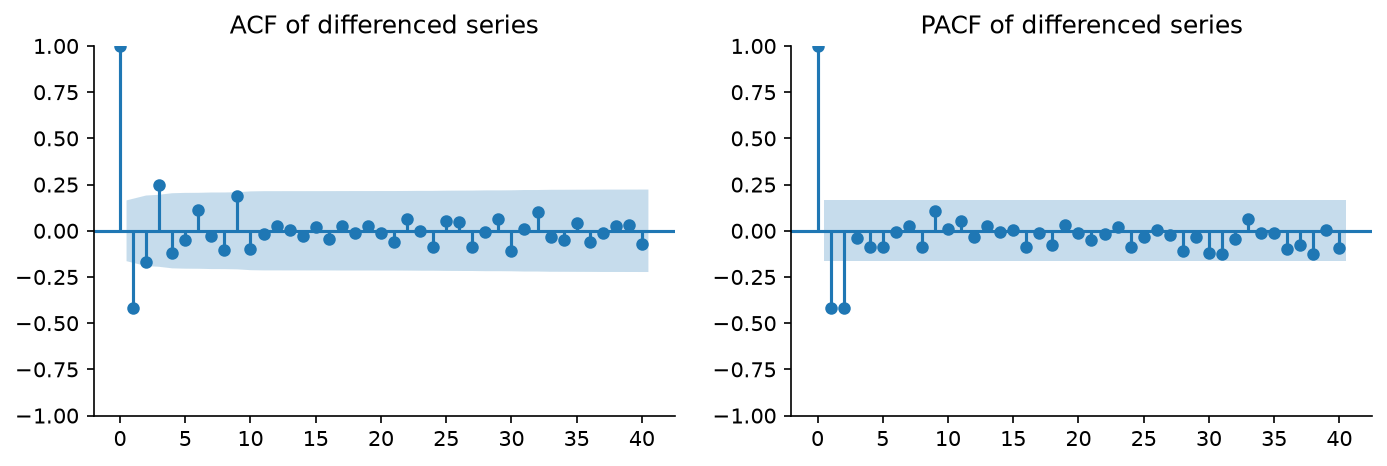
\includegraphics[width=\columnwidth]{f9_acf_pacf.png}
\caption{ACF and PACF of the first-differenced weekly series.}\label{fig:acf}
\end{figure} AIC selects ARIMA(2,1,1) with Fourier terms and a Tet dummy; the Tet effect is about $-61$ visits per week. The Ljung--Box test finds no remaining autocorrelation ($p=0.90$ at lag 10). On the 13-week test set (Table~\ref{tab:fc}, Fig.~\ref{fig:fc}), ARIMA achieves a MAPE of 5.8\% and all test points fall inside its 95\% interval, while Holt--Winters is slightly more accurate (4.5\%). Both beat the seasonal naive forecast (19.4\%), which cannot follow the clinic's growth. Refitted on all data, the model forecasts about 4{,}050 visits for Q1 2026, with a dip in Tet week.

\begin{table}[t]
\caption{Forecast accuracy, last 13 weeks of 2025}\label{tab:fc}
\centering\footnotesize
\begin{tabular}{@{}lrrr@{}}
\toprule
Model & MAE & RMSE & MAPE (\%)\\
\midrule
ARIMA(2,1,1) + Fourier & 16.2 & 19.2 & 5.75\\
Holt--Winters (additive) & \textbf{12.5} & \textbf{16.2} & \textbf{4.51}\\
Seasonal naive ($t-52$) & 52.4 & 55.2 & 19.38\\
\bottomrule
\end{tabular}
\end{table}

\begin{figure*}[t]
\centering
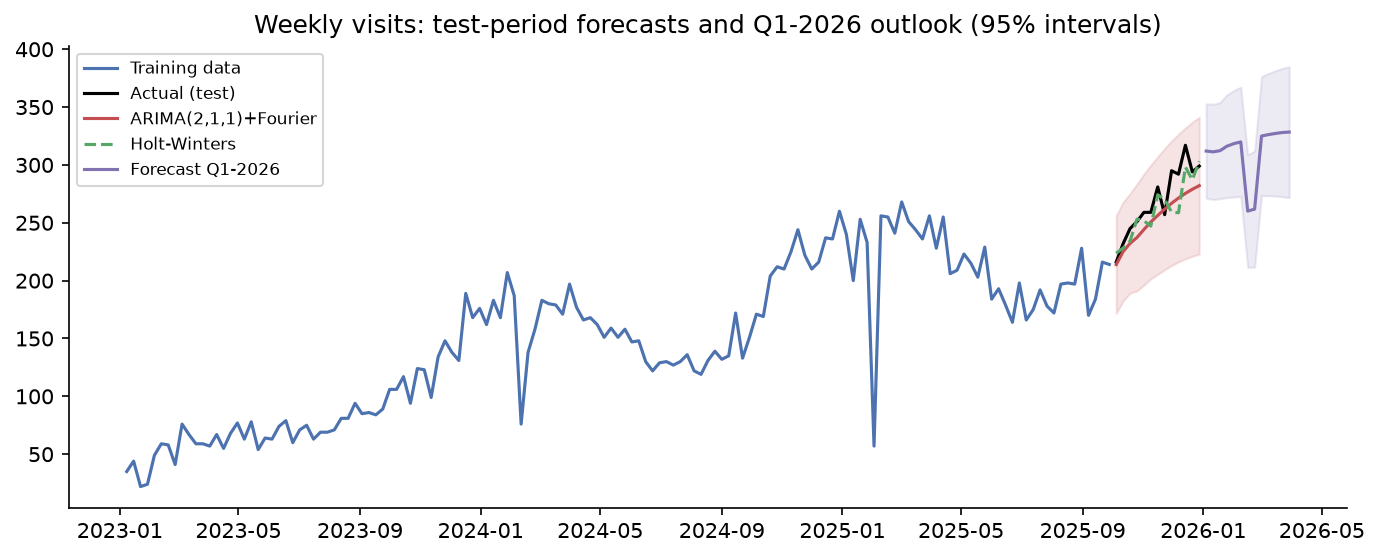
\includegraphics[width=0.9\textwidth]{f10_forecast.png}
\caption{Weekly visits with test-period forecasts and the Q1-2026 outlook (shaded: 95\% prediction intervals).}\label{fig:fc}
\end{figure*}

\subsection{Churn prediction}
Table~\ref{tab:ml} compares the four classifiers. All reach a cross-validated AUC between 0.876 and 0.887 with small standard deviations, so the differences are minor. Logistic regression has the highest CV AUC (0.887), test AUC (0.879) and specificity (0.84). The MLP neural network is the weakest on the test set. Permutation importance (Fig.~\ref{fig:roc}) shows that recency alone accounts for most of the predictive power (AUC drop 0.34), followed by visit frequency and chronic status. Waiting time and spending add little once recency is known.

\begin{table}[t]
\caption{Churn classifiers: 5-fold CV and test-set performance}\label{tab:ml}
\centering\footnotesize
\setlength{\tabcolsep}{3pt}
\begin{tabular}{@{}lrrrrrr@{}}
\toprule
Model & CV AUC & Test AUC & Acc. & Sens. & Spec. & F1\\
\midrule
Logistic reg. & \textbf{0.887} & \textbf{0.879} & \textbf{0.805} & 0.783 & \textbf{0.840} & 0.833\\
Random forest & 0.885 & 0.878 & 0.801 & \textbf{0.804} & 0.797 & \textbf{0.835}\\
Grad. boosting & 0.876 & 0.868 & 0.782 & 0.789 & 0.771 & 0.818\\
MLP (NN) & 0.879 & 0.859 & 0.767 & 0.757 & 0.784 & 0.802\\
\bottomrule
\end{tabular}
\end{table}

\begin{figure*}[t]
\centering
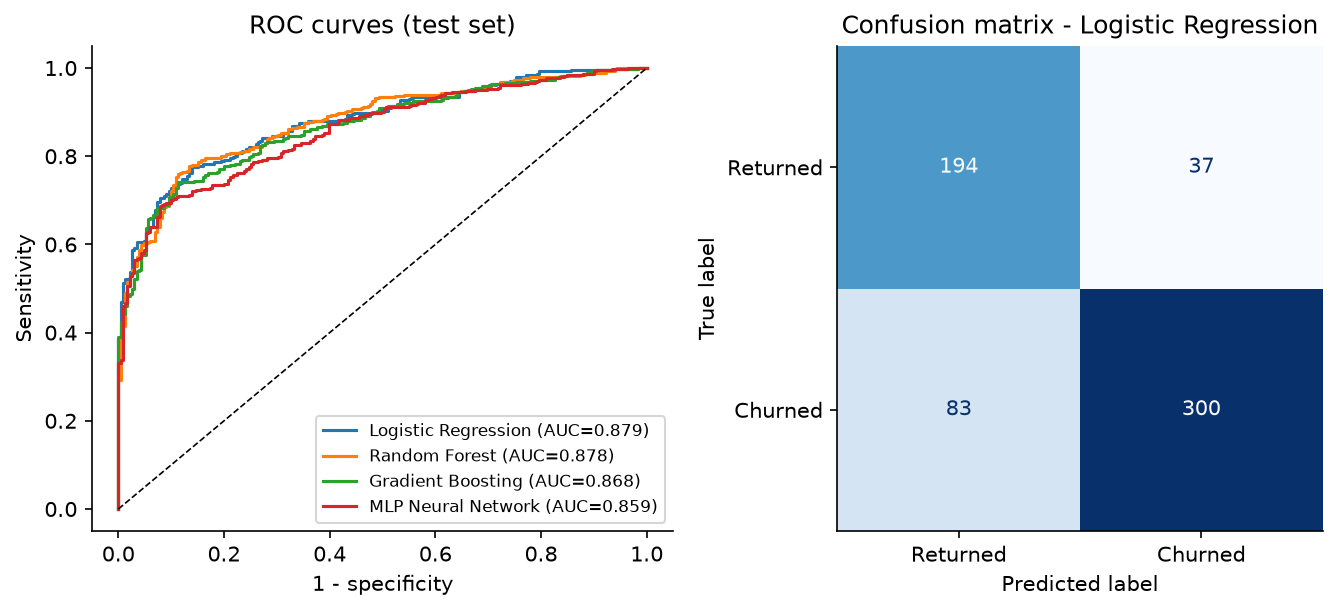
\includegraphics[width=0.62\textwidth]{f12_roc_confusion.png}\hfill
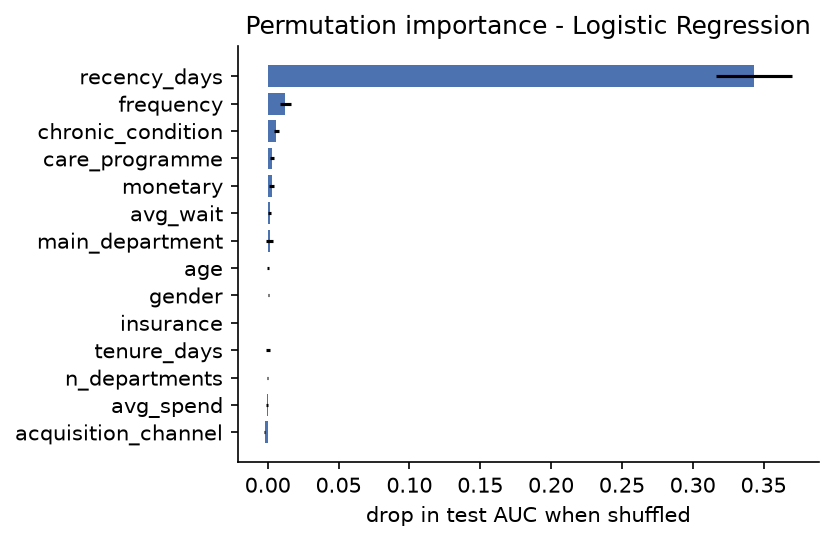
\includegraphics[width=0.36\textwidth]{f13_feature_importance.png}
\caption{Left: ROC curves and confusion matrix of the best model. Right: permutation importance (drop in test AUC).}\label{fig:roc}
\end{figure*}

%=====================================================================
\section{Discussion}\label{sec:discussion}
%=====================================================================
\subsection{Interpretation}
The six stages tell a consistent story. Value is concentrated: the top 10\% of predicted patients spend far more than the rest, and chronic and programme patients are worth most. Behaviour is driven mainly by \emph{recency}. A patient who has not visited for several months is very likely to be lost, and this one variable predicts churn almost as well as all the others combined. Experience matters through the satisfaction--loyalty chain. Doctor communication and service quality weigh more than price, and loyalty measured in the survey translates into actual return visits.

The model comparisons give two lessons. First, simple models were enough. Logistic regression matched tree ensembles and beat the neural network, in line with evidence that deep learning rarely dominates on small tabular data~\cite{grinsztajn2022,verbeke2012}. Second, the more complex ARIMA was slightly less accurate than Holt--Winters over a 13-week horizon. In both cases the simpler model is easier to explain to managers, which supports using it.

\subsection{Recommendations}
\textbf{For clinic management and marketing.} (i) Use the two-part PLV scores to rank patients and focus retention budgets on the top deciles. (ii) Trigger a reminder or follow-up call when a patient's recency passes about three months, since recency is the strongest churn signal. (iii) Promote the care programme to chronic patients: members spend more and return more often.

\textbf{For patient care.} (iv) Invest in doctor communication training and service consistency, the two largest drivers of satisfaction. (v) Reduce waiting time in General Medicine, the department with the longest waits, through scheduling. (vi) Staff according to the weekly forecast: add capacity for the January peak and reduce it in Tet week.

\subsection{Limitations}
The data are simulated. This makes ground-truth checks possible, but the effect sizes reflect our assumptions rather than real Vietnamese clinics, and the near-perfect SEM fit would not occur with real surveys. The survey sample is random, whereas real response is usually biased toward satisfied patients. The churn label uses a fixed 6-month window, and the models do not capture time-varying effects. Finally, predictive models applied to patients raise ethical questions about fairness and transparency~\cite{rajkomar2019}.

%=====================================================================
\section{Conclusion and Future Work}\label{sec:conclusion}
%=====================================================================
We built a reproducible pipeline that answers three key questions for a private clinic: who is valuable, what drives satisfaction, and how much demand to expect. It uses descriptive and inferential statistics, a two-part PLV regression, SEM, ARIMA and ML. On simulated data with known effects, every method recovered the true relations closely. Simple, interpretable models such as logistic regression and Holt--Winters performed as well as or better than complex ones. Future work will (1) apply the pipeline to real, anonymised clinic records; (2) add explainable-AI tools such as SHAP values for individual churn explanations; (3) model churn as time-to-event with survival analysis; and (4) audit the models for fairness across age, gender and insurance groups.

\section*{Data and Code Availability}
All code, data and figures are available at \url{https://github.com/Langl3y/STAT3013.R11.CTTT_Group10}. The full pipeline runs in under one minute with \texttt{python src/run\_all.py}.

\section*{AI Usage Statement}
An AI assistant (Claude, Anthropic) helped write code and draft parts of this paper. The author re-ran all analyses, verified every reported number against the generated output files, and revised the text. Details are given in the accompanying AI Usage Disclosure.

\bibliographystyle{IEEEtran}
\bibliography{refs}

\end{document}
